\documentclass[tikz,border=10pt]{standalone}
\usepackage{tikz}
\usepackage{amsmath}
\usetikzlibrary{calc,intersections}

\begin{document}

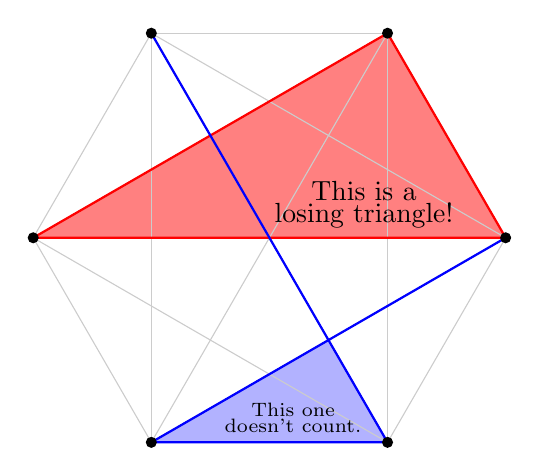
\begin{tikzpicture}
  % Define the radius of the hexagon
  \def\radius{3cm}

  % Define the vertices of the hexagon
  \foreach \i in {1,...,6} {
    \coordinate (V\i) at ({\radius*cos(60*(\i-1))}, {\radius*sin(60*(\i-1))});
  }

  % Name special paths
  \draw[name path=A] (V3)--(V6);
  \draw[name path=B] (V1)--(V5);

  % Define relevant intersection
  \path [name intersections={of=A and B,by=E}];

  % Create "Bad Triangle" region
  \draw[fill=blue!30!] (V6) -- (V5) -- (E) -- (V6);

  % Create "Good Triangle" region
  \draw[fill=red!50!] (V1) -- (V2) -- (V4) -- (V1);

  % Draw edges for the complete graph K6
  \foreach \i in {1,...,6} {
    \foreach \j in {\i,...,6} % slight improvement suggested by Japheth Wood
      \draw[black!20!] (V\i) -- (V\j);
    }

  % Draw special edges
` \draw[thick, red] (V1) -- (V2) -- (V4) -- (V1);
  \draw[thick, blue] (V3) -- (V6) -- (V5) -- (V1);

  % Draw the vertices
  \foreach \i in {1,...,6} {
    \fill (V\i) circle (2pt);
  }

  % Label good and bad triangles with text
  \node[above] at ($(V1)!0.3!(V4)$) {\Large $\substack{\text{This is a}\\\text{losing triangle!}}$};
  \node[above] at ($(V5)!0.6!(V6)$) {\normalsize $\substack{\text{This one}\\\text{doesn't count.}}$};

\end{tikzpicture}

\end{document}